\RequirePackage[orthodox]{nag}
\documentclass[11pt]{article}

%% Define the include path
\makeatletter
\providecommand*{\input@path}{}
\g@addto@macro\input@path{{include/}{../include/}}
\makeatother

\usepackage{../../include/akazachk}

\title{ECH4905 ChemE Optimization HW 1}
\author{Andres Espinosa}

\begin{document}
\maketitle

\section{Problem 1}
Consider the following matrix and perform the following calculations showing all your steps.
\begin{align*}
    A = 
  \begin{bmatrix}
     2 & 2 & 3 \\
     1 & -1 &0 \\
     -1 & 2 &1
  \end{bmatrix}
\end{align*}
\subsection{Part a}
Determinant of A
\\
\textbf{Solution: }
\begin{gather*}
    \det A = 
    2 (-1(1) - 0) - 2(1(1) + 0) + 3((1)(2) - (-1)(-1)) \\
    = -2 -2 + 6 - 3 \\
    \det A = -1
\end{gather*}

\subsection{Part b}
Eigenvalues and eigenvectors of A
\\
\textbf{Solution: }
\begin{gather*}
    (2- \lambda) ((-1 - \lambda)(1 - \lambda) - 0) - 2(1(1- \lambda) + 0) + 3((1)(2) - (-1-\lambda)(-1)) = 0 \\
    -(2-\lambda)(1+\lambda)(1-\lambda) -2(1-\lambda) + 6 -3(1+\lambda) = 0 \\
    -(2-\lambda)(1+\lambda)(1-\lambda) + (1-\lambda) \\
    (1-\lambda)((1+\lambda)(\lambda-2)+1) \\
    (1-\lambda)(\lambda^2 - \lambda -2 +1) \\
    (1-\lambda)(\lambda^2 - \lambda -1) \\
    \lambda = 1, \frac{1+\sqrt{5}}{2}, \frac{1 - \sqrt{5}}{2}
\end{gather*}

% Still need to do eigenvectors

\section{Problem 2}
Check if the set of all polynomials with real coefficients form a vector space.
\\
\textbf{Solution: }
%INSERT SOLUTION HERE

\section{Problem 3}
Consider the following function and perform the following calculations
\begin{equation*}
    f(x_1, x_2) = x_1^3 x_2 - x_1 x_2^3
\end{equation*}

\subsection{Part a}
Gradient of the function
\\
\textbf{Solution: }
\begin{align*}
    \nabla f(x_1, x_2) = 
  \begin{bmatrix}
     3x_1^2 x_2 - x_2^3 \\
     x_1^3 - 3x_1 x_2^2
  \end{bmatrix}
\end{align*}

\subsection{Part b}
Hessian of the function
\\
\textbf{Solution: }
\begin{align*}
    \nabla^2 f(x_1, x_2) = 
  \begin{bmatrix}
     6x_1 x_2 & 3x_1^2 - 3x_2^2 \\
     3x_1^2 - 3x_2^2 &  6 x_1 x_2
  \end{bmatrix}
\end{align*}

\subsection{Part c}
Write the second order Taylor expansions around a point $(x_1^*, x_2^*)$
\\
\textbf{Solution: }
% Still need to do this

\section{Problem 4}
Check if the following function is convex
\begin{equation*}
  f(x_1, x_2) = (1 - x_1)^2 + 100(x_2 - x_1^2)^2
\end{equation*}
\\
\textbf{Solution: }
In order to check if $f$ is convex, we calculate its hessian and evaluate if it is positive semi-definite.
\begin{align*}
  \nabla f(x_1, x_2) = 
  \begin{bmatrix}
    -2(1-x_1) - (2x_1) 200(x_2 - x_1^2) \\
    200(x_2 - x_1^2)
  \end{bmatrix}
  \\
  = 
  \begin{bmatrix}
    2x_1-2 - 400x_2 x_1 + 400x_1^3 \\
    200x_2 - 200x_1^2
  \end{bmatrix}
\end{align*}

\begin{align*}
  \nabla^2 f (x_1, x_2) =
  \begin{bmatrix}
    2 - 400x_2 + 1200 x_1^2 & -400 x_1 \\
    -400x_1 & 200
  \end{bmatrix}
\end{align*}
\begin{align*}
  (H- \lambda I) =
  \begin{bmatrix}
    2 - 400x_2 + 1200 x_1^2 - \lambda & -400 x_1 \\
    -400x_1 & 200 - \lambda
  \end{bmatrix}
  \\
  0 = (2 - 400x_2 + 1200 x_1^2 - \lambda)(200 - \lambda) - (-400 x_1) (-400 x_1) \\
  0 \leq 400 - 80,000 x_2 + 240,000 x_1^2 - 200 \lambda - 2 \lambda + 400 \lambda x_2 - 1200 x_1^2 \lambda + \lambda^2 - 160,000 x_1 ^2
\end{align*}
The function $f$ is convex when the above equation holds.
% Is this sufficient?
Another way to evaluate if the function $f$ is convex is by using rules that preserve convexity.
We can split $f$ into two functions $f = f_1 + f_2$.
\begin{equation*}
  f_1(x_1, x_2) = (1-x_1)^2, \quad f_2(x_1, x_2) = 100(x_2 - x_1^2)^2
\end{equation*}  
The non-negative weighted sum of two convex functions is convex so we break the problem down to verifying convexity of $f_1$ and $f_2$.
$f_1$ is clearly convex since it is a quadratic function in one variable.
To verify convexity of $f_2$, we can use composition rules.
\begin{equation*}
  f_2(x_1, x_2) = 100(\tilde{f}_2(x_1, x_2))^2, \quad \tilde{f}_2(x_1, x_2) = x_2 - x_1^2
\end{equation*}


The function $f_2$ is convex, non-increasing on $\tilde{f}_2(x_1, x_2) \leq 0$, and non-decreasing on $\tilde{f}_2(x_1, x_2) \geq 0$.
The function $\tilde{f}_2$ is concave, therefore the overall function $f$ is convex on the domain $\textbf{dom} f = x_2 - x_1^2 \leq 0$.



\section{Problem 5}
Check if the following function is convex
\begin{equation*}
  g(x_1, x_2) = 5 x_1^2 - 4x_1 x_2
\end{equation*}
\\
\textbf{Solution: }
Like the previous problem, we calculate the hessian of this function and evaluate when it is positive semi-definite.
\begin{align*}
  \nabla g(x_1, x_2) = 
  \begin{bmatrix}
    10 x_1 - 4 x_2 \\
    -4 x_1
  \end{bmatrix}
\end{align*}

\begin{align*}
  \nabla^2 g(x_1, x_2) = 
  \begin{bmatrix}
    10  & -4 \\
    -4 & 0
  \end{bmatrix}
\end{align*}

\begin{align*}
  (A - \lambda I) = 
  \begin{bmatrix}
    10 - \lambda  & -4 \\
    -4 & - \lambda
  \end{bmatrix}
  \\
  0 = (10- \lambda)(-\lambda) - (-4)(-4) \\
  0 = \lambda^2 - 10 \lambda - 16  \\
  16 + 25 = \lambda^2 - 10 \lambda + 25 \\
  (\lambda - 5)^2 = 41 \\
  \lambda - 5 = \pm \sqrt{41} \\
  \lambda = 5 \pm \sqrt{41} \\
  \lambda >= 0, \lambda <=0.
\end{align*}
Since we have one eigenvalue greater than 0 and one less than 0, the hessian is indefinite and $g$ is not convex.

\section{Problem 6}
Consider a set of linear equalities $Ax = b$ as well as a set of convex nonlinear inequalities $g(x) \leq 0$. 
Consider the feasible region constrained by these linear and nonlinear inequalities.
Assuming that this region is non-empty, show that this feasible region is convex.
\\
\textbf{Solution: }
% INSERT SOLUTION HERE

\section{Problem 7}
Consider the following optimization problem
\begin{align}
  \text{minimize} & \quad x_1 \\
  \text{subject to} & \quad x_1 + x_2 \leq 10 \\
  & \quad x_1 - 2x_2 \geq 1 \\
  & \quad x_1, x_2 \geq 0 \\
  & \quad x_1, x_2 \in \mathbb{R}
\end{align}

\subsection{Part a}
What type of problem is this (MILP, MINLP,...)? Justify.
\\
\textbf{Solution: }
This problem is an LP. The constraints are all linear and the variables are continuous variables in $\mathbb{R}$.

\subsection{Part b}
Draw the feasible region of the problem
\\
\textbf{Solution: }

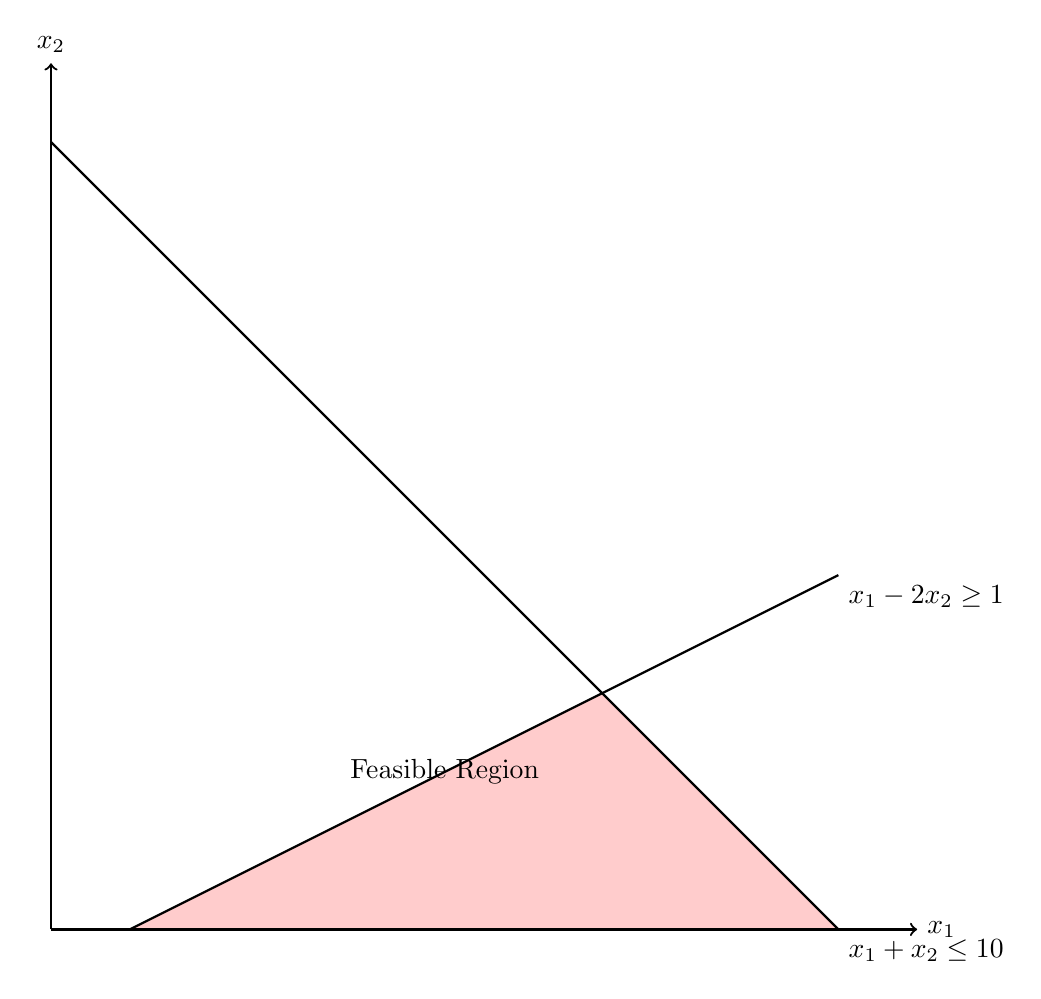
\begin{tikzpicture}
    \fill[red!20] (1,0) -- (10,0) -- (5,5) -- (7,3) -- cycle;
    \draw[thick, ->] (0,0) -- (11,0) node[right] {$x_1$};
    \draw[thick, ->] (0,0) -- (0,11) node[above] {$x_2$};
    \draw[thick] (0,10) -- (10,0) node[below right] {$x_1 + x_2 \leq 10$};
    \draw[thick] (1,0) -- (10,4.5) node[below right] {$x_1 - 2x_2 \geq 1$};
    \node at (5,2) {Feasible Region};
\end{tikzpicture}

\subsection{Part c}
Is the region convex or non-convex? Justify.
\\
\textbf{Solution: }
The problem is convex. 
The objective function is convex as it is linear. 
The feasible region is also convex because it is the intersection of half-spaces.
The feasible region is a polyhedron.

\section{Problem 8}Consider the following optimization problem
\begin{align}
  \text{minimize} & \quad x_1 \\
  \text{subject to} & \quad x_1 + x_2 \leq 10 \\
  & \quad x_1 - 2x_2 \geq 1 \\
  & \quad x_1, x_2 \geq 0 \\
  & \quad x_1, x_2 \in \mathbb{R}
\end{align}

\subsection{Part a}
What type of problem is this (MILP, MINLP, ...)? Justify.
\\
\textbf{Solution: }
This problem is a MILP. 
The constraints and objective function are all linear and the variables are binary integer variables.
Therefore it is not a standard LP, but instead an MILP.

\subsection{Part b}
Draw the feasible region of the problem.
\\
\textbf{Solution: }

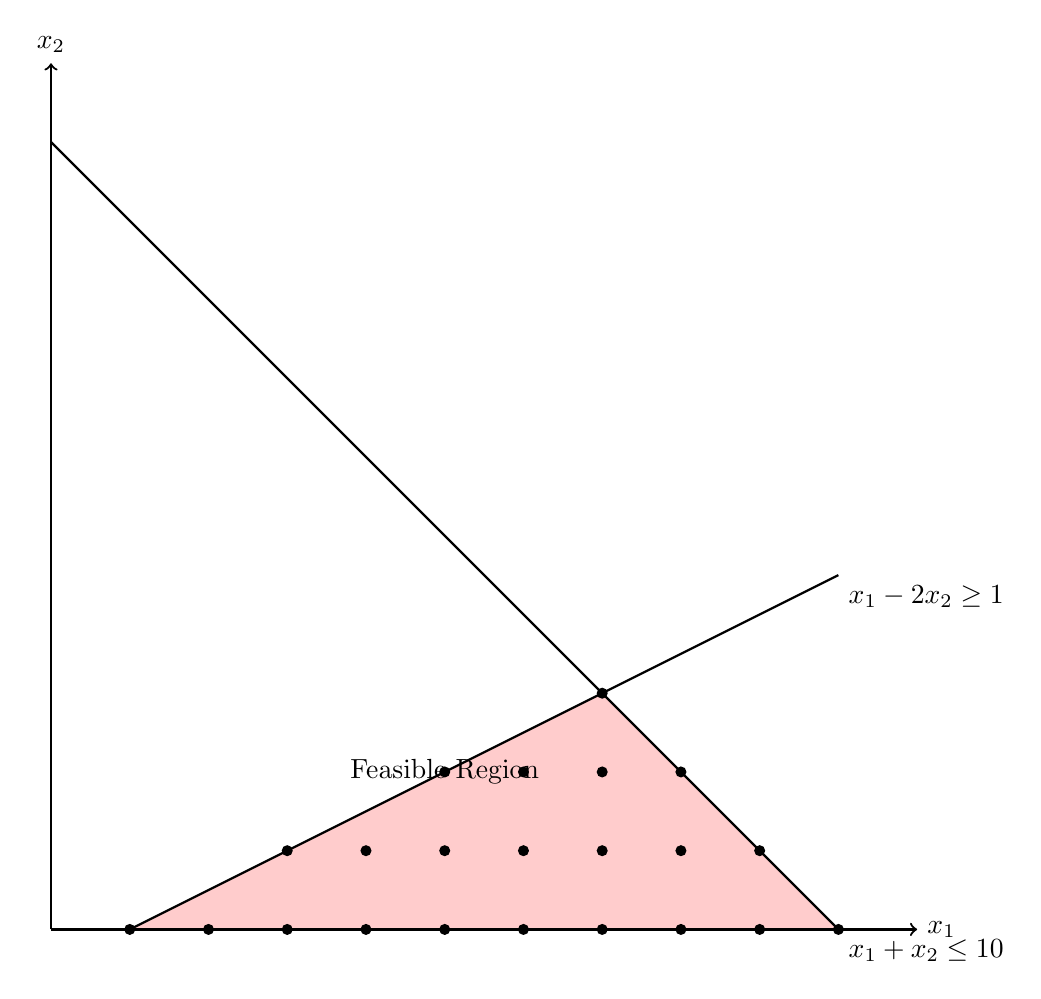
\begin{tikzpicture}
    % Shaded feasible region - keep as is to show the feasible region
    \fill[red!20] (1,0) -- (10,0) -- (5,5) -- (7,3) -- cycle;

    % Axes
    \draw[thick, ->] (0,0) -- (11,0) node[right] {$x_1$};
    \draw[thick, ->] (0,0) -- (0,11) node[above] {$x_2$};

    % Constraints
    \draw[thick] (0,10) -- (10,0) node[below right] {$x_1 + x_2 \leq 10$};
    \draw[thick] (1,0) -- (10,4.5) node[below right] {$x_1 - 2x_2 \geq 1$};

    % Feasible region label
    \node at (5,2) {Feasible Region};

    % Manually mark specific points
    \def\markpoint(#1,#2){
                \fill (#1,#2) circle (2pt);
    }

    % Mark several points manually
    \markpoint(1,0)
    \markpoint(2,0)
    \markpoint(3,0)
    \markpoint(4,0)
    \markpoint(5,0)
    \markpoint(6,0)
    \markpoint(7,0)
    \markpoint(8,0)
    \markpoint(9,0)
    \markpoint(10,0)
    \markpoint(3,1)
    \markpoint(4,1)
    \markpoint(5,1)
    \markpoint(6,1)
    \markpoint(7,1)
    \markpoint(8,1)
    \markpoint(9,1)


    \markpoint(5,2)
    \markpoint(6,2)
    \markpoint(7,2)
    \markpoint(8,2)
  
 
    \markpoint(7,3)
   



\end{tikzpicture}

\subsection{Part c}
Is the region convex or non-convex? Justify.
\\
\textbf{Solution: }

The problem is non-convex because there are integer variables. 
The disjoint that integer variables introduce naturally make the problem non-convex.


\end{document}